\documentclass[a4paper,12pt]{report}
\usepackage[utf8]{inputenc}
\usepackage[francais]{babel}
\usepackage{fancyhdr}
\usepackage{graphicx}
\usepackage{tikz}
\usetikzlibrary{calc}
\usepackage{listings}
\usepackage{xcolor}
\definecolor{grey}{rgb}{0.9,0.9,0.9}
\usepackage{titlesec}
\usepackage{verbatim}
\usepackage{listings}
\usepackage{textcomp}
\usepackage{hyperref}
\usepackage{longtable}
\usepackage{colortbl}
\usepackage{amssymb}


\frenchbsetup{StandardLists=true}
\newcommand{\marge}{18mm}
\usepackage[left=\marge,right=\marge,top=\marge,bottom=\marge]{geometry}
\pagestyle{fancy}
\setlength{\headheight}{14pt}
\chead{
  \textbf{Binôme :} Douaille Erwan 
    \hspace{2em}
  \textbf{Groupe :} M1 Info TI}
\renewcommand{\headrulewidth}{1pt}
\linespread{1}
\setlength{\columnseprule}{0.2pt}
\definecolor{javakeyword}{rgb}{0,0,0.5}
\definecolor{javastring}{rgb}{0,0.5,0}
\definecolor{javacomment}{rgb}{0.5,0.5,0.5}
\lstdefinestyle{Scilab}{
   language=Scilab, basicstyle=\footnotesize,       % the size of the fonts that are used for the code
  numbers=left,                   % where to put the line-numbers
  numberstyle=\tiny\color{gray},  % the style that is used for the line-numbers
  stepnumber=1,                   % the step between two line-numbers. If it's 1, each line
                                  % will be numbered
  numbersep=5pt,                  % how far the line-numbers are from the code
  backgroundcolor=\color{white},  % choose the background color. You must add \usepackage{color}
  showspaces=false,               % show spaces adding particular underscores
  showstringspaces=false,         % underline spaces within strings
  showtabs=false,                 % show tabs within strings adding particular underscores
  frame=single,                   % adds a frame around the code
  rulecolor=\color{black},        % if not set, the frame-color may be changed on line-breaks within not-black text (e.g. commens (green here))
  tabsize=2,                      % sets default tabsize to 2 spaces
  captionpos=b,                   % sets the caption-position to bottom
  breaklines=true,                % sets automatic line breaking
  breakatwhitespace=false,        % sets if automatic breaks should only happen at whitespace
  title=\lstname,                 % show the filename of files included with \lstinputlisting;
   stringstyle=\color{javastring},
   keywordstyle=\color{javakeyword}\ttfamily\textbf,
   commentstyle=\color{javacomment}\ttfamily\textit
 }
 

\begin{document}



\makeatletter
\begin{titlepage}
\centering
\vspace{-10em}
{\LARGE \textbf{\textsc{Rapport de Projet RVI}}}\\
\vspace{3em}

\includegraphics[scale=0.6]{image/thalassa.png}\\
\vspace{3em}
{\LARGE \textsc{Projet Thalassa: simulation de plongée sous-marine}}\\

\vspace{8em}
Par\\
\vspace{1em}
{\LARGE \@author}\\

\vspace{2em}



\begin{tikzpicture}[remember picture,overlay]

\node [below left,xshift=-1cm, yshift=4cm] at (current page.south east){
\includegraphics[scale=0.6]{image/ustl1.png}};

\end{tikzpicture}
\end{titlepage}
\makeatother

\sloppy

\setcounter{page}{1} 
\newpage

\section*{Introduction}
Dans ce tp, nous allons voir la procédure décrite par \textit{Zhengyou Zhang} pour calibrer une caméra grâce à une mire. Nous comprendrons l'utilité des matrices \textit{d'homographies}, \textit{intrinsèques} et \textit{extrinsèques} et verrons comment les calculer, coder avec Scilab.

\section*{Analyse du code source et du rapport de \textit{Zhengyou Zhang} }


\textit{Zhengyou Zhang}dans son rapport définit plusieurs étapes pour calibrer une caméra:

\begin{itemize}
	\item estimation d'une matrice d'homographie, qui permettra de faire des transformation linéaire entre deux plans.
	\item estimation de la matrice intrinsèque, qui contient les données propres aux paramètres optiques de la caméra
	\item estimation de la matrice extrinsèque, qui permet de déterminer la rotation et la position de la caméra dans l'espace 3D
\end{itemize}

Nous remarquons que dans le programme qui nous est fournit nous retrouvons bien ces 3 parties:


\begin{lstlisting}[style=Scilab]
... 
for i = 1:ni                             
  m(1:2,:,i) = read('points-'+string(i)+'.txt', -1, 2)';
  m(3,:,i) = ones(1, np);
  // Estimer l'homographie entre la mire et l' image
  H(:,:,i) = ZhangHomography(M(sansZ,:), m(:,:,i));
  V = [V; ZhangConstraints(H(:,:,i))];
end

...

// Estimations des matrices intrinseques
A = IntrinsicMatrix(b);
iA = inv(A);

// Estimations des matrices extrinseques
E = zeros(3, 4, ni);
for i = 1:ni
  E(:,:,i) = ExtrinsicMatrix(iA, H(:,:,i));
end
\end{lstlisting}

\section*{Complétion des méthodes et analyse des résultats}

Une fois avoir compris les différentes étapes de la calibration de caméra, il nous a été demandé de coder certaines méthodes.

La méthode \textit{ZhangConstraintTerm} a été codé en fonction de la formule du rapport de \textit{Zhengyou Zhang}: 

\textit{vij = [hi1hj1, hi1hj2 + hi2hj1, hi2hj2, hi3hj1 + hi1hj3, hi3hj2 + hi2hj3, hi3hj3]T}


\begin{lstlisting}[style=Scilab]
function v = ZhangConstraintTerm(H, i, j)
    v = [H(1,i)*H(1,j), (H(1,i)*H(2,j))+(H(2,i)*H(1,j)), H(2,i)*H(2,j),(H(3,i)*H(1,j))+(H(1,i)*H(3,j)), (H(3,i)*H(2,j))+(H(2,i)*H(3,j)),H(3,i)*H(3,j) ];
endfunction
\end{lstlisting}


La seconde méthode à compléter est la méthode déterminant les paramètres intrinsèques de la caméra. Selon le rapport de \textit{Zhengyou Zhang} voici les formules permettant d'obtenir cette matrice intrinsèque:

\begin{figure}[!ht]
	\center
	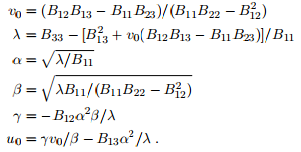
\includegraphics[scale=1]{./image/intrinsequeForm.png}
\end{figure}

Voici la méthode \textit{IntrinsicMatrix} obtenue: 

\begin{lstlisting}[style=Scilab]
function A = IntrinsicMatrix(b)
    vo = (b(2)*b(4)-b(1)*b(5))/(b(1)*b(3)-b(2)*b(2));
    lambda = b(6)-(b(4)*b(4)+vo*(b(2)*b(4)-b(1)*b(5)))/b(1);
    alpha = sqrt(lambda/b(1));
    bet= sqrt(lambda*b(1)/(b(1)*b(3)-b(2)*b(2)));
    delta = -b(2)*alpha*alpha*bet/lambda;
    uo = (delta*vo/bet-b(4)*alpha*alpha/lambda);
    A = [alpha,lambda,uo;0,bet,vo;0,0,1];
endfunction
\end{lstlisting}
\textit{Alpha} et \textit{bet} représentent la distance focale, \textit{u0} et \textit{v0} indique le point dit central de l'image et lambda représente la non-orthogonalité potentielle des lignes du capteur.

Une fois ces méthodes écrites il nous est maintenant possible de comparer nos résultats avec les résultats obtenus dans les script povray qui nous sont fournis.

\begin{center}
\[
	povray=\left (
	\begin{array}{ccc}
		3546.099291 & 0.000000    & 320.000000    \\
		0.000000    & 3546.099291 & 240.000000   \\
		0.000000    & 0.000000    & 1.000000    \\
	\end{array}
	\right )
\]
\[
	nosResultats=\left (
	\begin{array}{ccc}
		3498.2767 & 0.9869483 & 336.76583 \\
        0 & 3503.8946 & 220.1142 \\
        0 & 0 & 1.0 \\
	\end{array}
	\right )	
\]
\end{center}

On observe que nos valeurs sont très proches des valeurs fournis dans le script povray. La différence est négligeable. Cette différence apparait probablement par le calcul de la matrice intrinsèque. En effet nous connaissons certains paramètres de la caméra et ces valeurs, qui seront fixes, pourraient corriger ce problème de différences.

Une fois cette matrice intrinsèque calculée il nous est possible de déterminer les matrices extrinsèques pour chaque images.

La matrice extrinsèque se compose de plusieurs parties qui sont trois vecteurs de rotations et un vecteur de translation.

La matrice extrinsèque se détermine par les calculs suivants:

\begin{figure}[!ht]
	\center
	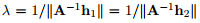
\includegraphics[scale=1]{./image/lambdaForm.png}\\
	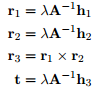
\includegraphics[scale=1]{./image/extrinsequeForm.png}
\end{figure}

A$^{-1}$ étant l'inverse de notre matrice intrinsèque.
Voici le résultat de notre fonction \textit{ExtrinsicMatrix} en Scilab:

\begin{lstlisting}[style=Scilab]
function E = ExtrinsicMatrix(iA, H)
    lambda = 1/abs(iA*H(:,1));
    lambda = lambda(1);
    r1 = lambda * iA * H(:,1);
    r2 = lambda * iA * H(:,2);
    r3 = CrossProduct(r1,r2);
    t = lambda * iA * H(:,3);

    E  = [r1,r2,r3,t];
endfunction
\end{lstlisting}

En observant les résultats que nous obtenons aux résultats dans les \textit{images-i.txt} on remarque une fois de plus que ces valeurs sont très  proches. Pour le vecteur translation les valeurs \textit{-48} et \textit{54} peuvent surprendre mais au final ces valeurs sont faibles si on compare au \textit{10000} appliqué sur l'axe z.


\begin{center}
\[
	image-1=\left (
	\begin{array}{cccc}
		0.0 & 0.0 & 0.0 & 0.0    \\
		0.0 & 0.0 & 0.0 & 0.0  \\
		0.0 & 0.0 & 0.0 & 10000  \\
	\end{array}
	\right )
\]
\[
	extrinseque1=\left (
	\begin{array}{cccc}
		 1.      &   - 0.0002699 & - 0.0006686 & - 48.876008  \\
    0.0000377  &  0.9982951  &  0.0015761  &  54.733323  \\
    0.0006696 & - 0.0015763  &  0.9982951   & 9854.3632
	\end{array}
	\right )
\]
\end{center}

Seul les résultats de l'image 1 sont içi cités mais l'observation est la même pour les autres images.

\section*{Simplification de la méthode de Zhang}

En modifiant la méthode déterminant les matrices intrinsèques en passant en paramètres les paramètres connus, il est présenté dans le rapport que cela aura une influence sur les résultats. Le calcul de tout les paramètres intrinsèques introduise certaines erreurs. Cela est dûe au bruit.

Comme prévue l'introduction de données réelles influent sur le calcul et fourniront de meilleurs résultats.

\newpage

\section*{Conclusion}

Dans ce tp, nous avons utilisé les méthodes de \textit{Zhang} pour obtenir la matrice homographe, les matrices intrinsèques et extrinsèques. Nous avons également observé leurs comportements en comparant des résultats théoriques à ceux obtenus sur des images données. La simplification de la méthode de Zhang laisse à suposer que nos résultats auraient été plus proches des résultats théoriques.


\end{document}